
\begin{figure*}
	\centering
	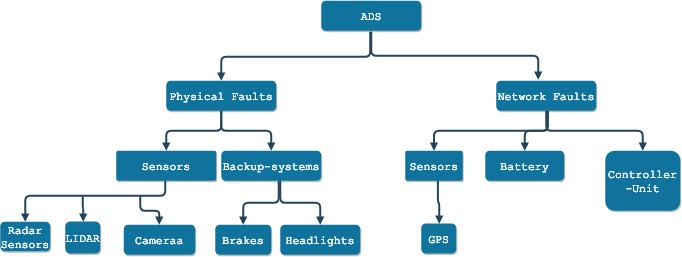
\includegraphics[width=0.7\linewidth]{Fault-modelgeneral}
	\caption[Fault-model for ADS]{This shows a general fault model of Autonomous Driving Systems. We have kept it generic enough to be considered for different Autonomous systems. However, our work is oriented towards autonomous cars.}
	\label{fig:fault-modelgeneral}
\end{figure*}
\section{Background}
\subsection{ Autonomous Cars}
Self-driving autonomous cars use various autonomous technologies to provide an effortless mode of transportation. In order for autonomous cars to work effectively a proper synchronization of advanced sensors collecting data from surrounding environments and advanced algorithms processing data and the vehicle in real-time.

% Main components of self-driving car
The main components of a self-driving car are sensors ( we will talk about them in more details in the next subsection), computer processors, batteries, back-up systems ( eg. steering, braking etc.), rounded-shapes which maximizes the sensors coverage area and the interiors( designed for riding, not for driving). 

\subsection{Sensors}
Sensors are the core components in a self-driving car. We will talk about them in a little more detail, since our research goal is to find error rate in self-driving cars caused by sensor faults.

%Major sensors
The core sensors of a self-driving car are as follows:
\subsubsection{Radar sensors}
Radar sensors help the autonomous vehicles in determining the road dynamics such as detours, collisions, navigation by sending signals to the on-board processor. The on-board processor on receiving the signals from the radar sensors takes decisions such as applying brakes and/or move out of the way. The decisions made by the processor or the brain of the vehicle don't depend entirely on the radar sensors. The processor decision also depends on the gyroscopes and  wheel encoders to send accurate and on time signals to it. The radar sensors are usually mounted on the bumper ( two in the front and two in the back).

\subsubsection{Optics}
High powered cameras in conjunction with Radar sensors are another vital component of the autonomous vehicles. The camera setup on each car differs according to the manufacturer. The main goal of the camera placement is to get the surrounding views covered properly, so that the processor can take correct decisions. Some manufacturers use a single camera on the windshield ~\cite{singlecamera} whereas some vehicles require multiple cameras placed equidistant from each other to get overlapped views which are sent to the processor. The processor uses the views to calculate the depth of the field and/or perform semantic segmentation.

\subsubsection{GPS}
Global Positioning Sensors is very similar to the navigation maps we use in our mobile phones. However, GPS in autonomous vehicles is very important since we enter the destination point and the start point of our trip. The GPS works in conjunction with LIDAR, Radar Sensors and Deep learning software ~\cite{GPS} in order to guide the vehicle in the correct direction to reach the destination.

\subsubsection{LIDAR}
Laser Illuminating Detection and Ranging is the sensor on which we are focusing on in this work. LIDAR unit resembles a spinning siren light and ranges up-to 100 meters. The goal of LIDAR is to provide driver-less cars with accurate long range detection. LIDAR continuously performs 360 degree rotation in order to scan the world around. The sensor generates raw information about the world and the information is sent to the processor which digs out the relevant information in order to guide the vehicle and take decisions.

\subsection{LIDAR}
Since we are trying to determine the failure rates of LIDAR, we give a brief overview of how LIDAR units work in an autonomous car.

%LiDAR working
The autonomous car LIDAR units follow four steps in order to function:
\begin{enumerate}
	\item The LIDAR unit which is continuously rotating emits a laser beam generated by the laser emitter present inside LIDAR.
	\item The laser bounces off the an object. The object is usually something solid and the moment, laser hits the first solid object it bounces off and returns to LIDAR.
	\item The gathered light is then bounced downwards to the receiver, where the light is interpreted. 
	\item This is a continuous process in all directions and the data gets sent to the processor which generates a map of its surroundings.
\end{enumerate}